%%%%%%%%%%%%%%%%%%%%%%%%%%%%%%%%%%%%%%% Exponential Decay


\begin{figure}[H]
\centering
\begin{subfigure}[t]{0.5\textwidth}
  \centering
  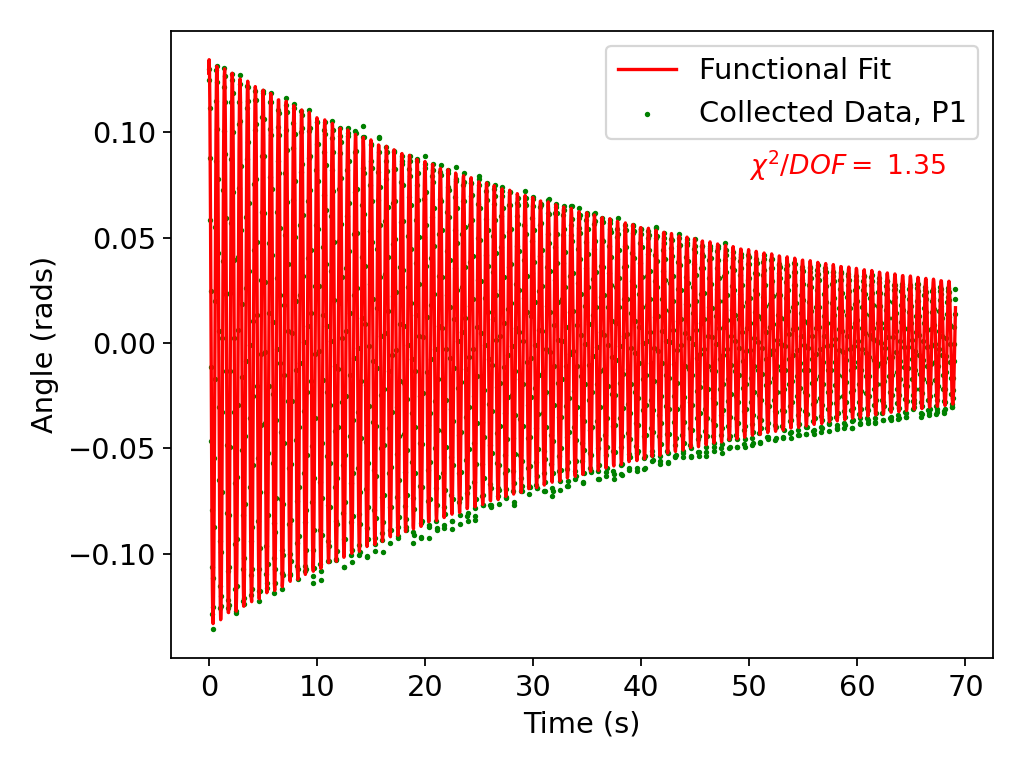
\includegraphics[width=1\textwidth]{Plots/P1.png}
  \caption{\small{$m = 0.10\text{kg}$, $L = 0.10\text{m}$, $\theta_0 = 0.13\text{rads}$}}
  \label{exponential_decay1}
\end{subfigure}%
\begin{subfigure}[t]{.5\textwidth}
  \centering
  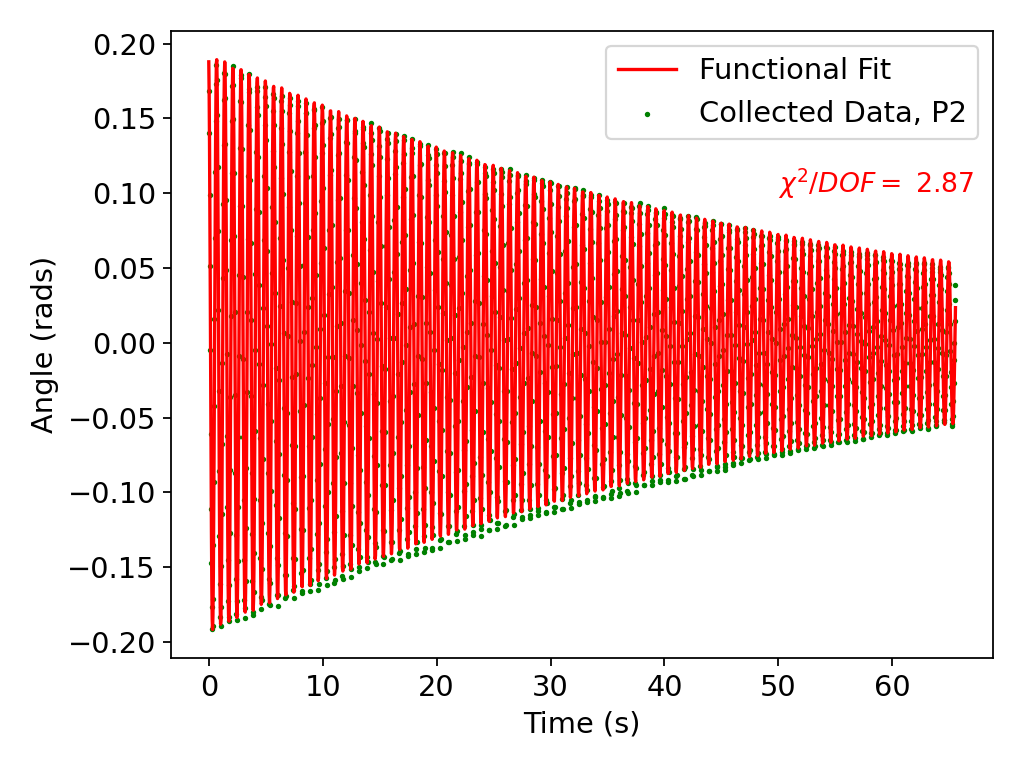
\includegraphics[width=\textwidth]{Plots/P2.png}
  \caption{\small{$m = 0.10\text{kg}$, $L = 0.10\text{m}$, $\theta_0 = 0.19\text{rads}$ }}
  \label{exponential_decay2}
\end{subfigure}
\caption{\small{Plots of two sets of data which visually display the exponential decay of the amplitude of the pendulum as time evolves. The respective functional fits have a decay constant of $\tau_1 = (76.06\pm 2.81)s$ and $\tau_2 = (51.35 \pm 0.28) s$.}}
\end{figure}


\begin{table}[h!]
\centering
\caption{A table displaying the values of the quotient of $\tau/T$ for all of the data sets. In each column, the indicated independent variable is change, while all others are remained fixed. Note that each of the values of the ratios are numbers; these are unitless quantities used entirely for the purpose of gaining numerical estimations on the efficiency of the system. Note that only five data sets were collected where the length and mass are left fixed, while there are fix data sets with distinct angles.} 
\begin{tabular}{ |c|c|c|c|c|c|c| }
\hline
Independent Variable & Data Set 1 & Data Set 2 & Data Set 3 & Data Set 4 & Data Set 5 & Data Set 6 \\ 
\hline
Mass $m$ $[\text{kg}]$ & $99.73 \pm 4.33$ & $103.19 \pm 2.95$ & $135.45 \pm 7.07$ & $130.47 \pm 5.96$ & $174.21 \pm 5.16$ & N/A\\
\hline
 Length $L$ $[\text{m}]$ & $73.52 \pm 2.81$ & $103.23 \pm 2.95$ & $138.32 \pm 6.20$ & $197.06 \pm 11.09$ & $186.16 \pm 13.12$ & N/A\\
\hline
Amplitude $\theta_0$ [\text{rads}] & $63.13 \pm 0.33$ & $71.91\pm 0.28$ & $80.77\pm3.34$ & $89.91\pm1.64$ & $57.12\pm0.46$ & $24.32\pm0.18$\\
\hline
\end{tabular}
\label{decay coeff table}
\end{table}
\normalsize




%%%%%%%%%%%%%%%%%%%%%%%%%%%%%%%%%%%%%%% Length versus Tau

\pagebreak
\large{\textbf{Length $\ell$ Versus Decay Coefficient $\tau$}}\normalsize\\[0.20cm]



\begin{figure}[H]
\centering
\begin{subfigure}[t]{0.5\textwidth}
  \centering
  \includegraphics[width=1\textwidth]{Plots/length_vs_tau_residual1.png}
  \caption{\small{Residuals of quadratic fit for length versus decay coefficient}}
  \label{length_tau_residual1}
\end{subfigure}%
\begin{subfigure}[t]{.5\textwidth}
  \centering
  \includegraphics[width=\textwidth]{Plots/length_vs_tau_residual2.png}
  \caption{\small{Residuals of linear fit for length versus decay coefficient}}
  \label{length_tau_residual2}
\end{subfigure}
\caption{\small{Residual plots denoting the residuals between the period versus $\tau$ points in Figure \ref{length_tau} and the two functional forms fitted to the data.}}
\end{figure}


%%%%%%%%%%%%%%%%%%%%%%%%%%%%%%%%%%%%%%% Mass versus Tau








\Large{\textbf{Decay Coefficient $\tau$}}\normalsize\\[0.20cm]


\large{\textbf{Mass $m$ and Amplitude $\theta_0$ Versus Decay Coefficient $\tau$}}\normalsize\\[0.20cm]



\begin{figure}[H]
\centering
\begin{subfigure}[t]{0.5\textwidth}
  \centering
  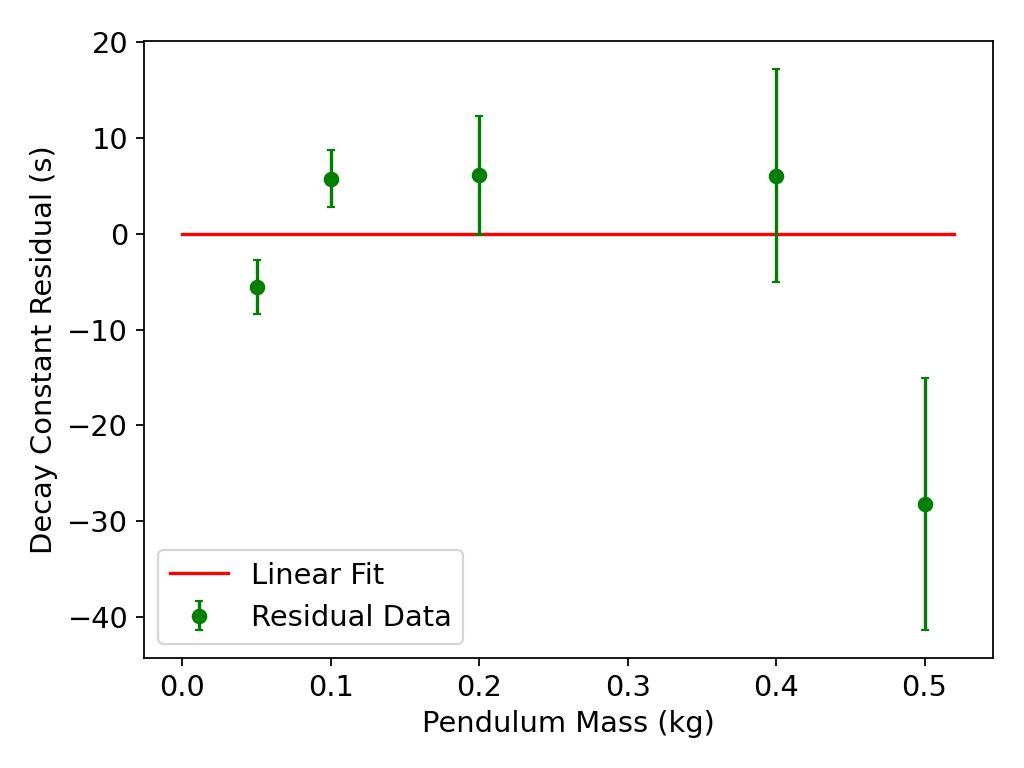
\includegraphics[width=1\textwidth]{Plots/masses_vs_tau_residual.png}
  \caption{\small{Residuals of linear fit.}}
  \label{mass_tau_residual1}
\end{subfigure}%
\begin{subfigure}[t]{.5\textwidth}
  \centering
  \includegraphics[width=\textwidth]{Plots/masses_vs_tau_residual2.png}
  \caption{\small{Residuals of quadratic fit.}}
  \label{mass_tau_residual2}
\end{subfigure}
\caption{\small{Residual plots denoting the residuals between the mass versus $\tau$ points in Figure \ref{mass_tau} and the two functional forms fitted to the data.}}
\end{figure}



%%%%%%%%%%%%%%%%%%%%%%%%%%%%%%%%%%%%%%% Theta_0 versus Tau


\begin{figure}[H]
\centering
\begin{subfigure}[t]{0.5\textwidth}
  \centering
  \includegraphics[width=1\textwidth]{Plots/theta_vs_tau_residual1.png}
  \caption{\small{Residuals of linear fit.}}
  \label{theta_tau_residual1}
\end{subfigure}%
\begin{subfigure}[t]{.5\textwidth}
  \centering
  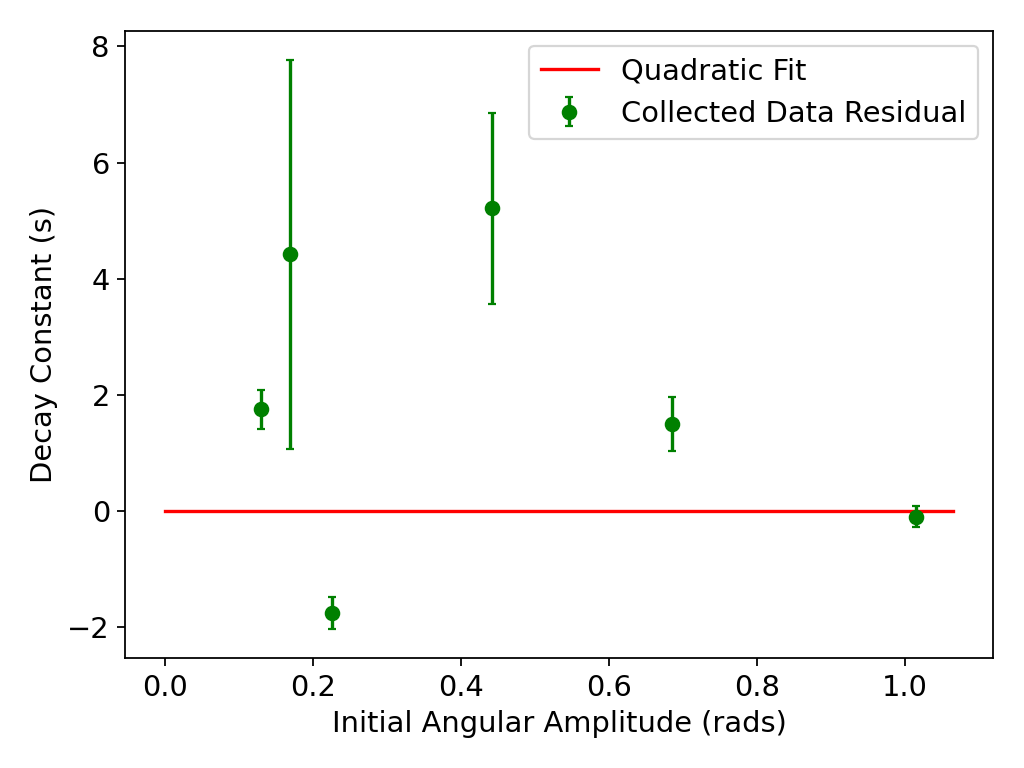
\includegraphics[width=\textwidth]{Plots/theta_vs_tau_residual2.png}
  \caption{\small{Residuals of quadratic fit.}}
  \label{theta_tau_residual2}
\end{subfigure}
\caption{\small{Residual plots denoting the residuals between the initial angular amplitude versus $\tau$ points in Figure \ref{eq: theta_vs_tau} and the two functional forms fitted to the data.}}
\end{figure}








%%%%%%%%%%%%%%%%%%%%%%%%%%%%%%%%%%%%%%% Symmetry


\begin{figure}[H]
\centering
\begin{subfigure}[t]{0.5\textwidth}
  \centering
  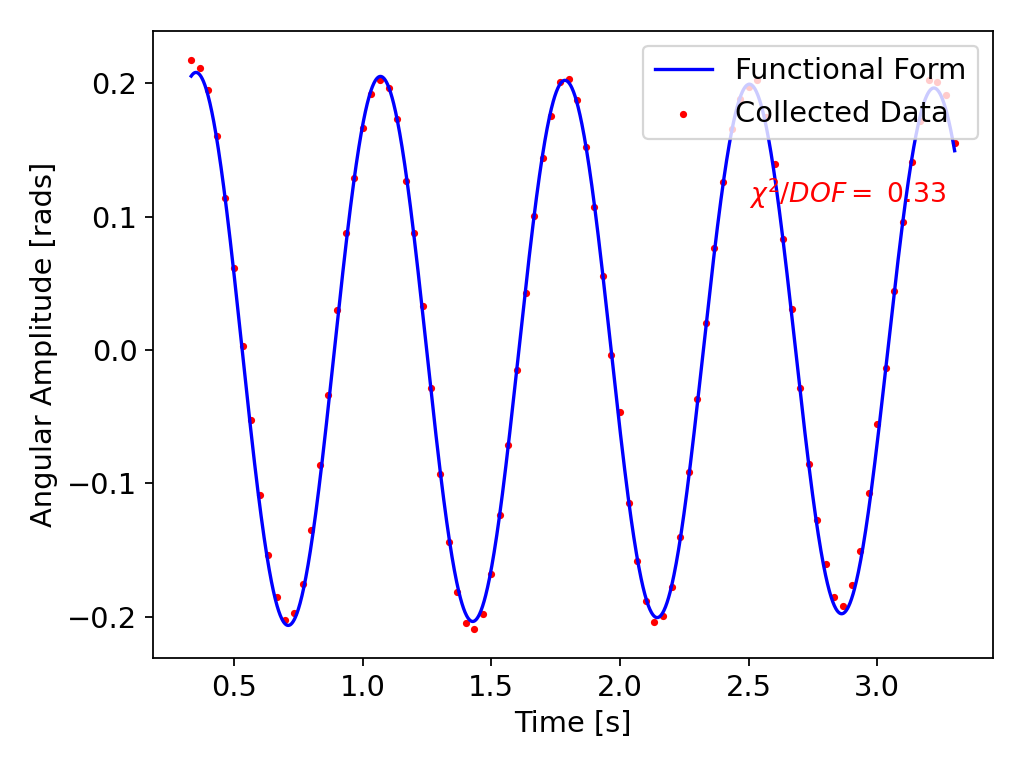
\includegraphics[width=1\textwidth]{Plots/symmetry_plot.png}
    \caption{\small{$L = 0.1\text{m}$, $m = 0.1\text{kg}$, and $\theta_0 = 0.22\text{rads}$.}}
  \label{symmetry}
\end{subfigure}%
\begin{subfigure}[t]{.5\textwidth}
  \centering
  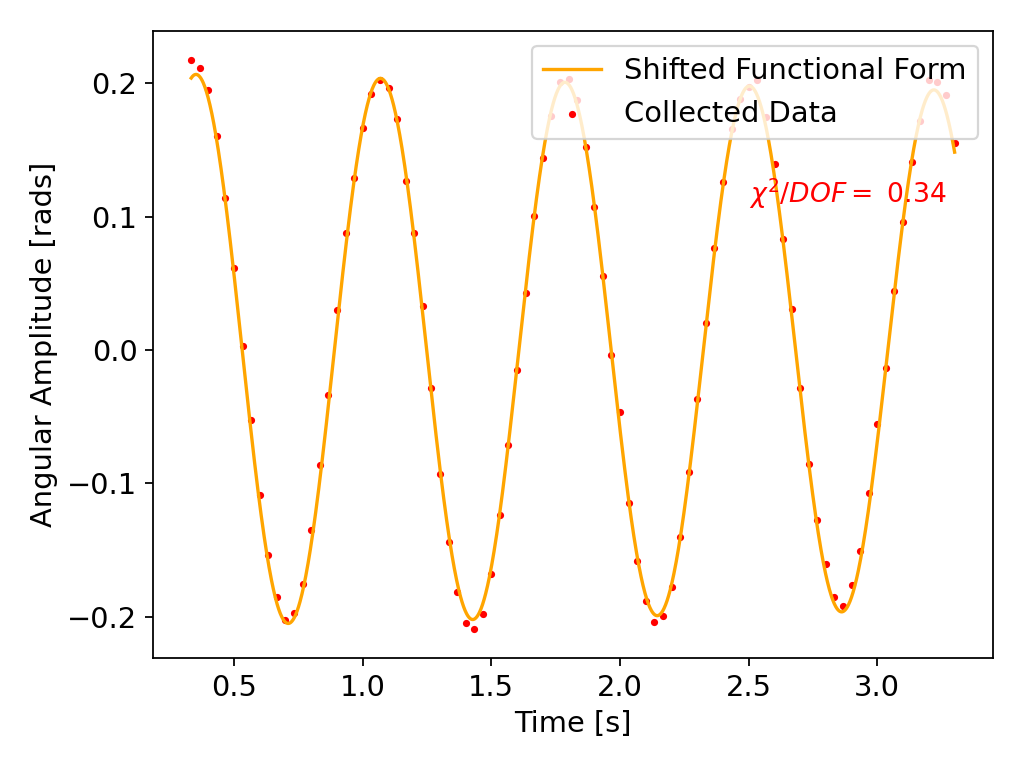
\includegraphics[width=\textwidth]{Plots/symmetry_shifted.png}
    \caption{\small{$L = 0.1\text{m}$, $m = 0.1\text{kg}$, and $\theta_0 = 0.22\text{rads}$.}}
  \label{symmetry_shifted}
\end{subfigure}
\caption{\small{Two plots of the first 100 data points of the pendulum with independent variables as stated above. Figure \ref{symmetry} includes a functional fit of the form of Eq.(\ref{theta equation}) and is printed with it's associated goodness of fit estimation. Figure \ref{symmetry_shifted} contains the exact same functional form, but shifted a value $T/2 = (0.36\pm 0.0012)\text{s}$, and mirrored across the $t$ axis.}}
\end{figure}


\begin{figure}[H]
\centering
\begin{subfigure}[t]{0.5\textwidth}
  \centering
  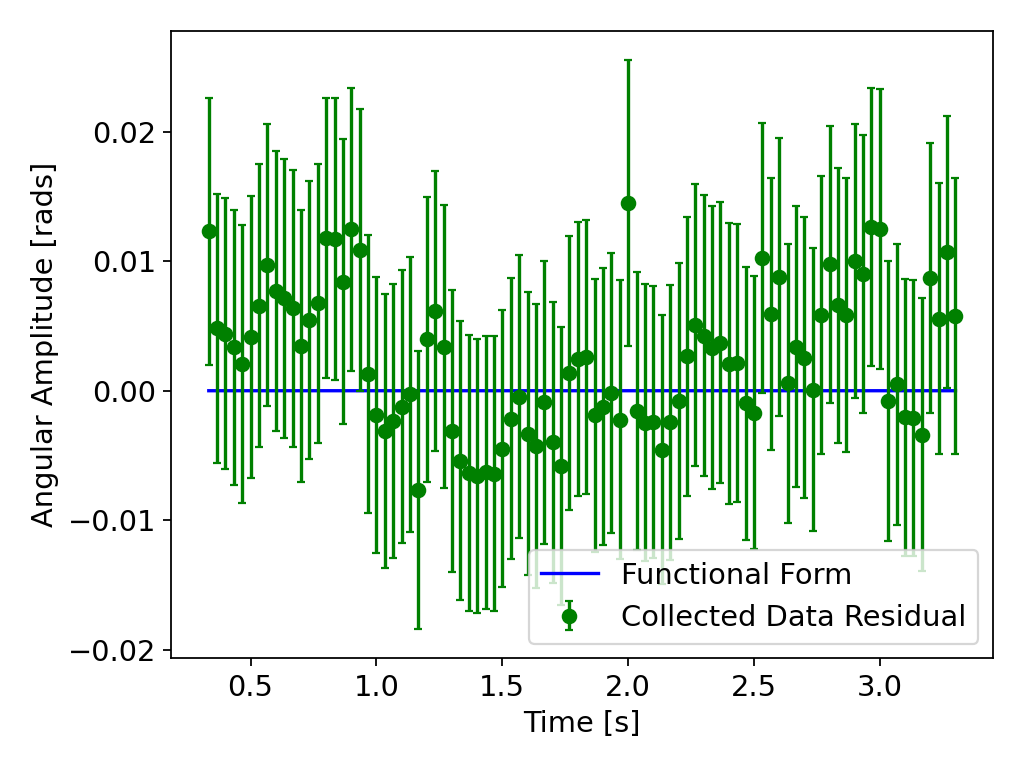
\includegraphics[width=1\textwidth]{Plots/symmetry_plot_residual.png}
  \caption{\small{Residuals of collected data in Figure \ref{symmetry}.}}
  \label{symmetry_residual}
\end{subfigure}%
\begin{subfigure}[t]{.5\textwidth}
  \centering
  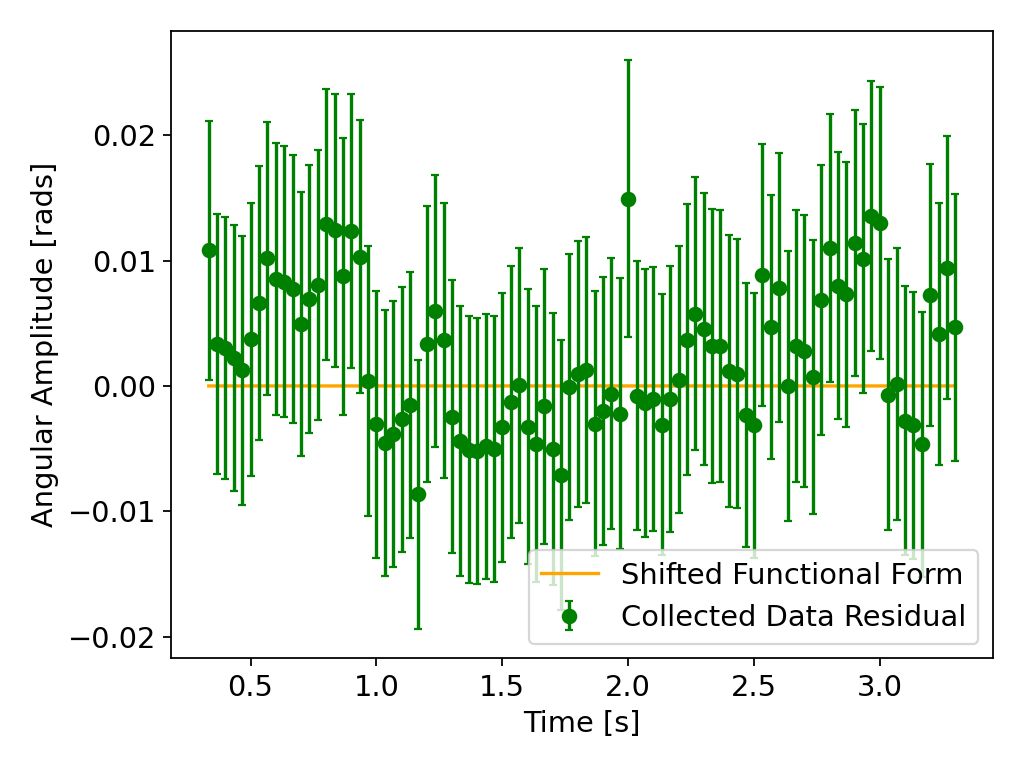
\includegraphics[width=\textwidth]{Plots/symmetry_shifted_residual.png}
  \caption{\small{Residuals of collected data in Figure \ref{symmetry_shifted}.}}
  \label{symmetry_shifted_residual}
\end{subfigure}
\caption{\small{Residual plots of the data in Figures \ref{symmetry} and \ref{symmetry_residual} against the fitted functional form and the shifted functional form respectively.}}
\end{figure}







%%%%%%%%%%%%%%%%%%%%%%%%%%%%%%%%%%%%%%% Data Plots

\large{\textbf{Raw Data Plots}}\normalsize\\[0.20cm]

\begin{figure}[H]
\centering
\begin{subfigure}[t]{0.5\textwidth}
  \centering
  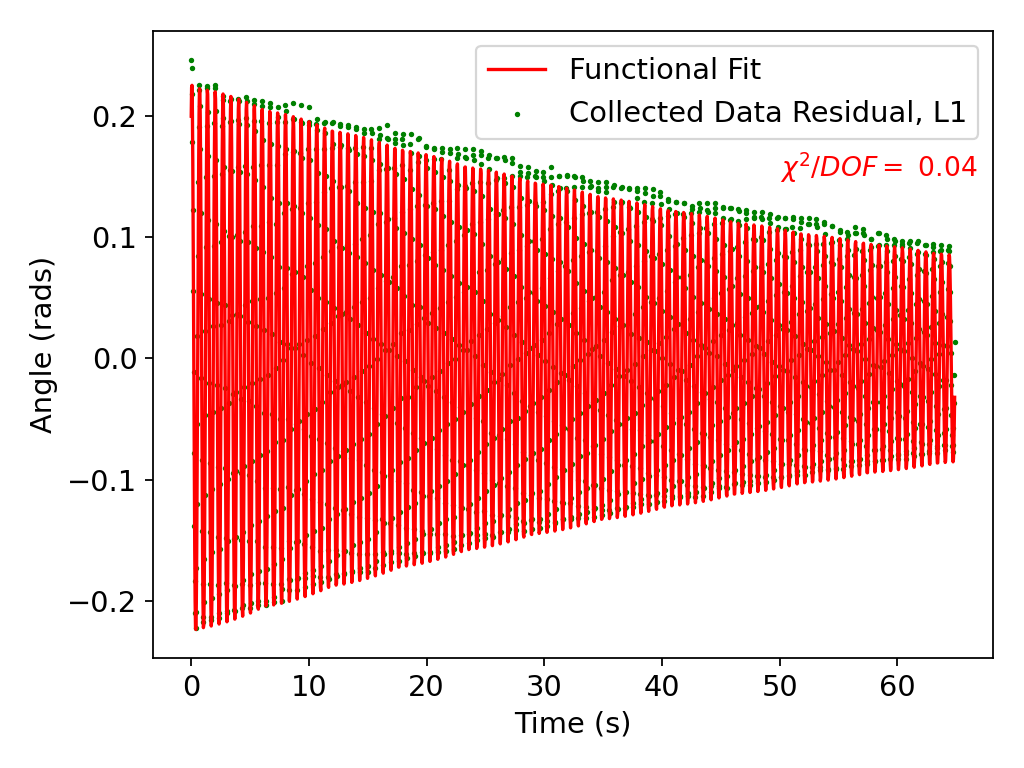
\includegraphics[width=1\textwidth]{Plots/L1.png}
  \caption{\small{$L = 0.075\text{m}$, $m = 0.10\text{kg}$, $\theta_0 = 0.22\text{rads}$}}
  \label{L1}
\end{subfigure}%
\begin{subfigure}[t]{.5\textwidth}
  \centering
  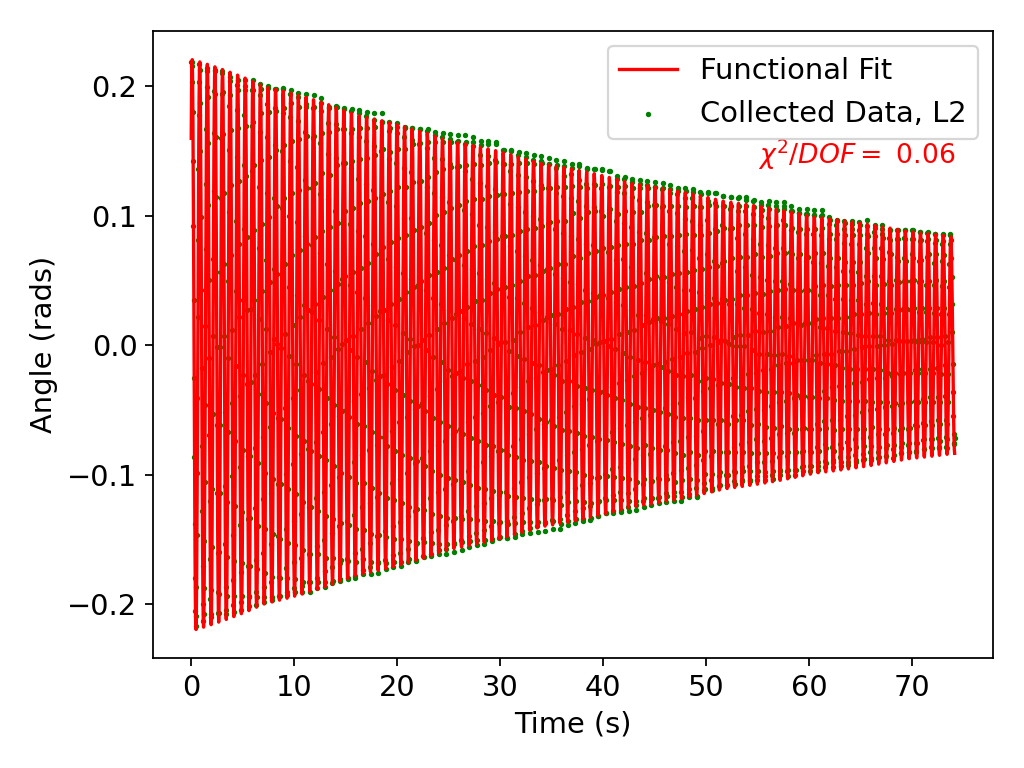
\includegraphics[width=\textwidth]{Plots/L2.png}
  \caption{\small{$L = 0.10\text{m}$, $m = 0.10\text{kg}$, $\theta_0 = 0.22\text{rads}$}}
  \label{L2}
\end{subfigure}
\caption{\small{Plots of the angular amplitude versus time for two systems with independent variables specified above plotted alongside an optimized function of the form Eq.(\ref{theta equation}). Each data set includes over 1 full minute of behaviour of the pendulum.}}
\end{figure}


\begin{figure}[H]
\centering
\begin{subfigure}[t]{0.5\textwidth}
  \centering
  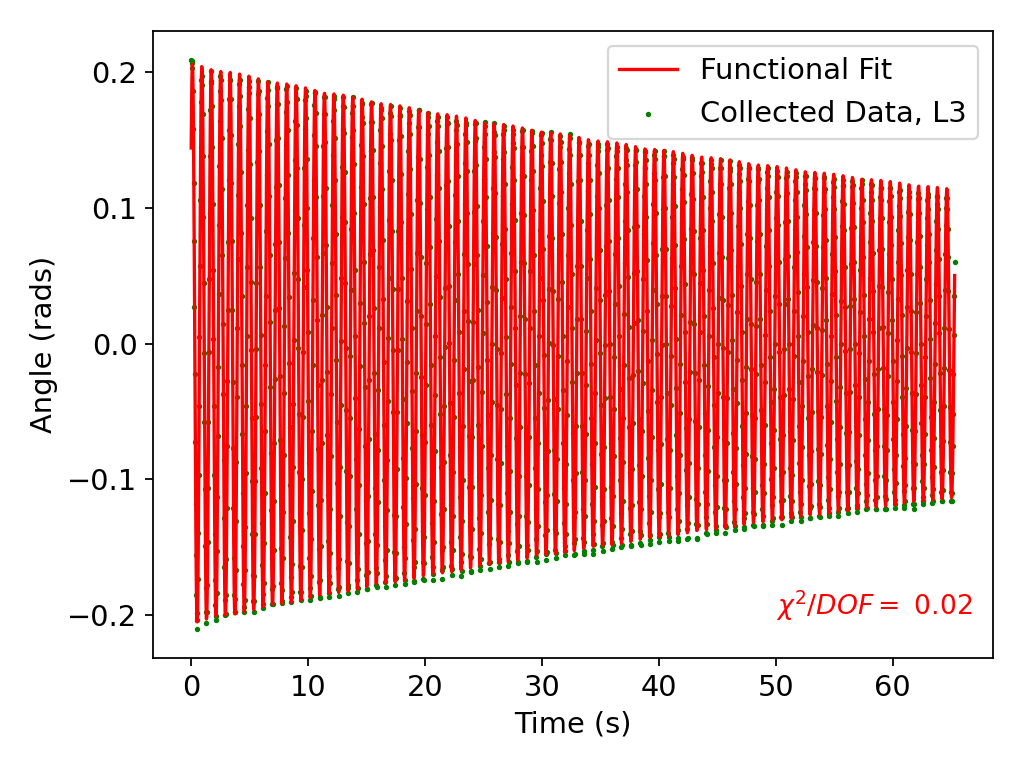
\includegraphics[width=1\textwidth]{Plots/L3.png}
  \caption{\small{$L = 0.125\text{m}$, $m = 0.10\text{kg}$, $\theta_0 = 0.22\text{rads}$}}
  \label{L3}
\end{subfigure}%
\begin{subfigure}[t]{.5\textwidth}
  \centering
  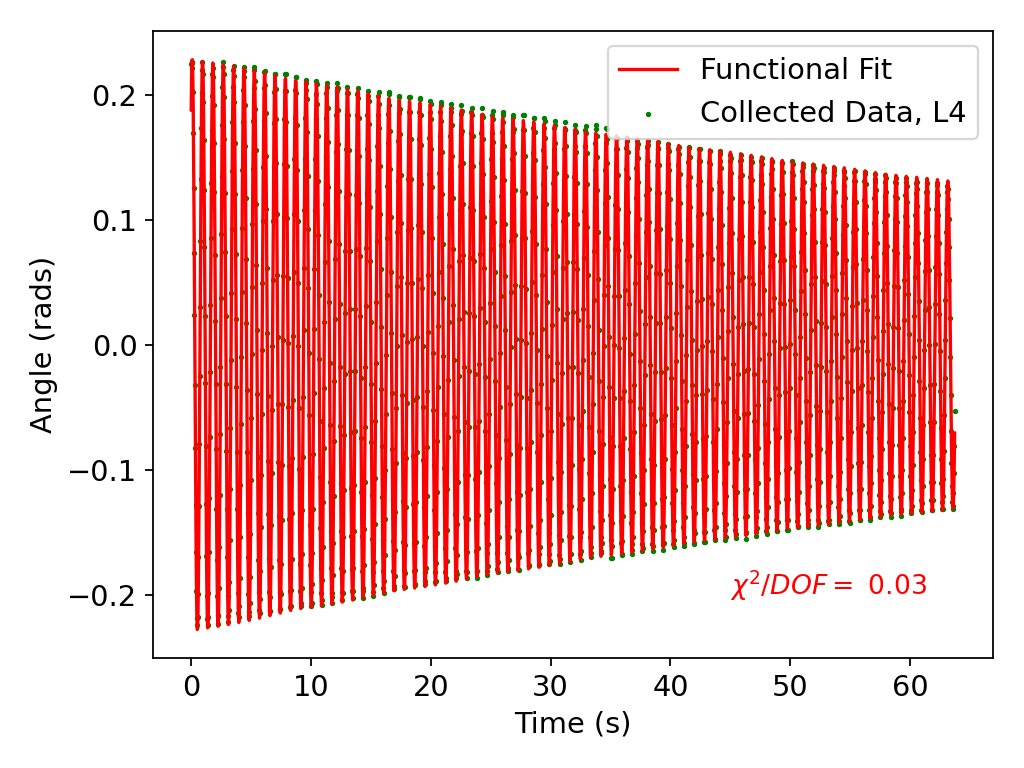
\includegraphics[width=\textwidth]{Plots/L4.png}
  \caption{\small{$L = 0.15\text{m}$, $m = 0.10\text{kg}$, $\theta_0 = 0.22\text{rads}$}}
  \label{L4}
\end{subfigure}
\caption{\small{Plots of the angular amplitude versus time for two systems with independent variables specified above plotted alongside an optimized function of the form Eq.(\ref{theta equation}). Each data set includes over 1 full minute of behaviour of the Plots.}}
\end{figure}


\begin{figure}[H]
\centering
\begin{subfigure}[t]{0.5\textwidth}
  \centering
  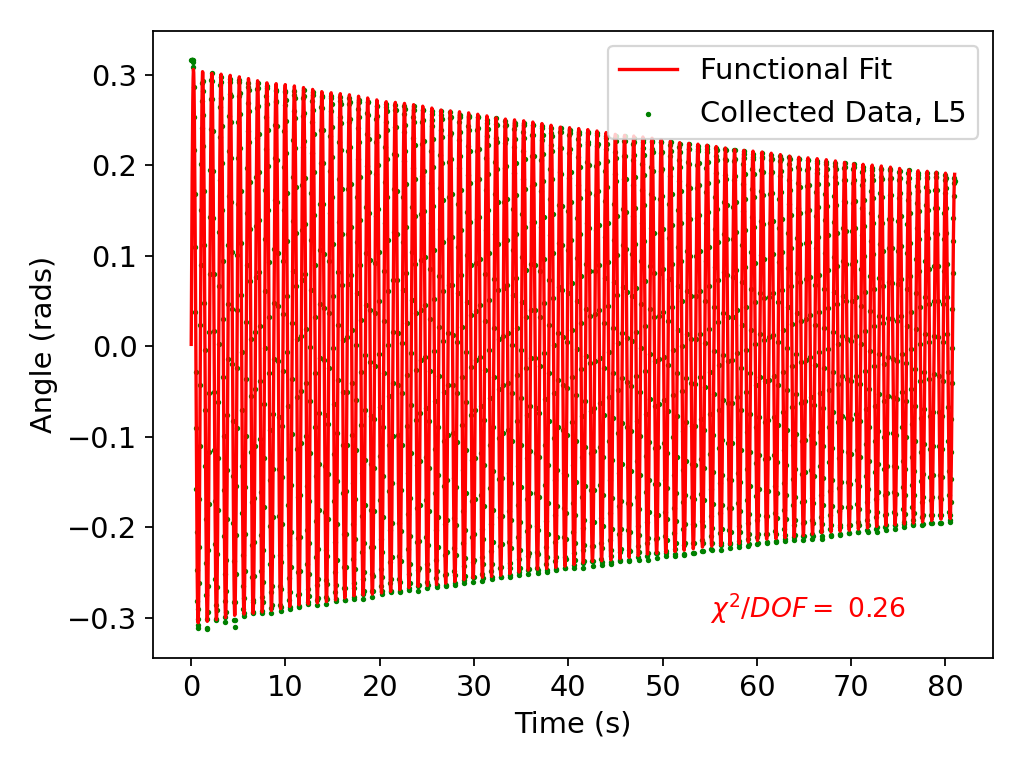
\includegraphics[width=1\textwidth]{Plots/L5.png}
  \caption{\small{$L = 0.20\text{m}$, $m = 0.10\text{kg}$, $\theta_0 = 0.22\text{rads}$}}
  \label{L5}
\end{subfigure}%
\begin{subfigure}[t]{.5\textwidth}
  \centering
  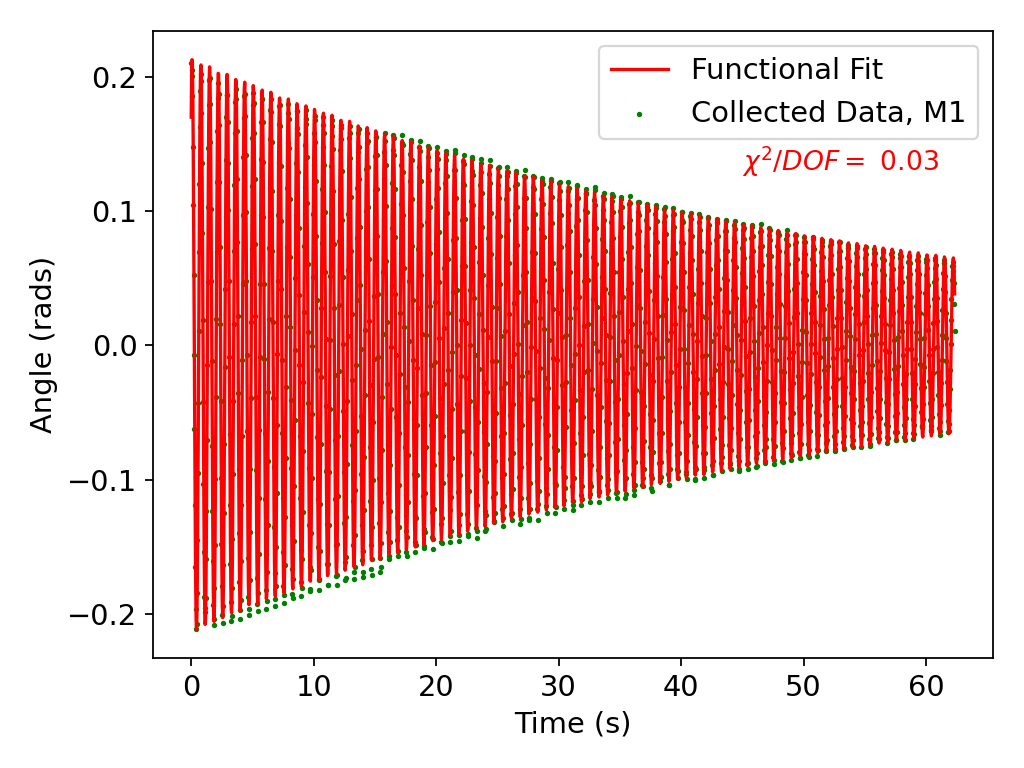
\includegraphics[width=\textwidth]{Plots/M1.png}
  \caption{\small{$L = 0.10\text{m}$, $m = 0.05\text{kg}$, $\theta_0 = 0.22\text{rads}$}}
  \label{M1}
\end{subfigure}
\caption{\small{Plots of the angular amplitude versus time for two systems with independent variables specified above plotted alongside an optimized function of the form Eq.(\ref{theta equation}). Each data set includes over 1 full minute of behaviour of the pendulum.}}
\end{figure}

\begin{figure}[H]
\centering
\begin{subfigure}[t]{0.5\textwidth}
  \centering
  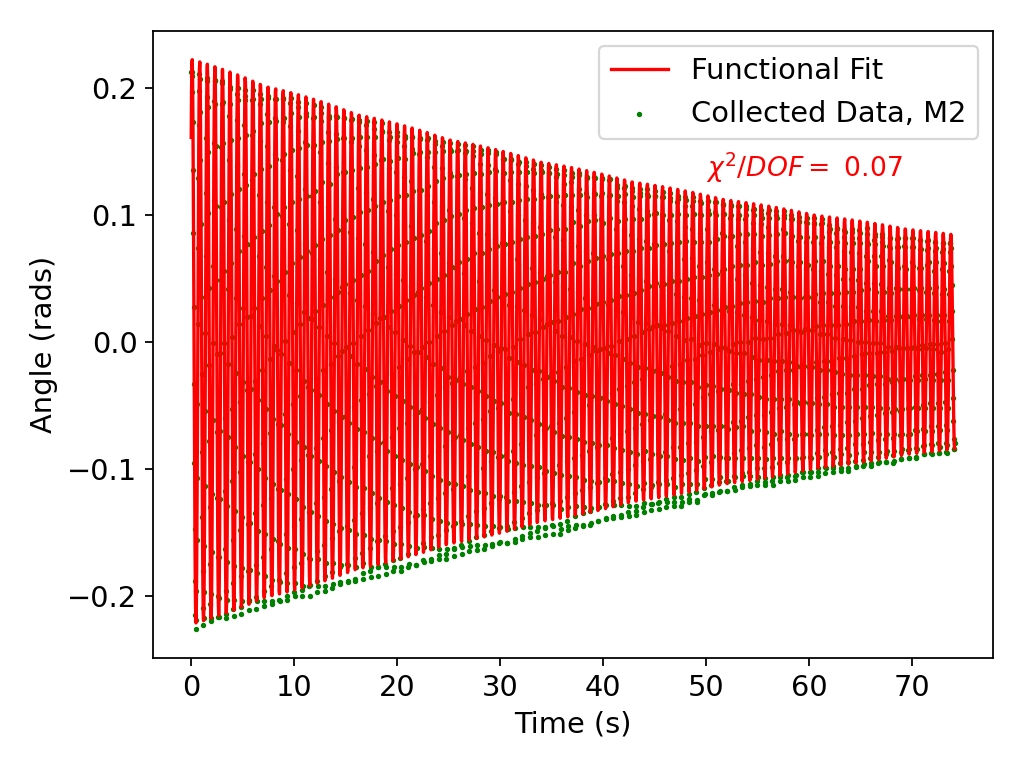
\includegraphics[width=1\textwidth]{Plots/M2.png}
  \caption{\small{$L = 0.10\text{m}$, $m = 0.10\text{kg}$, $\theta_0 = 0.22\text{rads}$}}
  \label{M2}
\end{subfigure}%
\begin{subfigure}[t]{.5\textwidth}
  \centering
  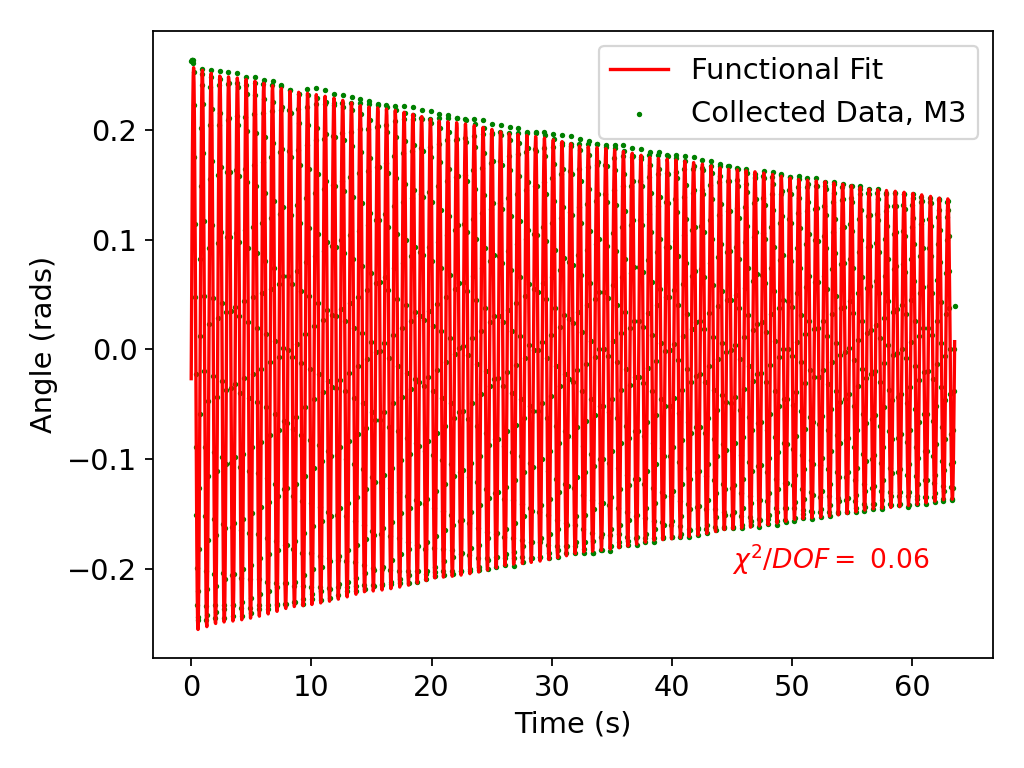
\includegraphics[width=\textwidth]{Plots/M3.png}
  \caption{\small{$L = 0.10\text{m}$, $m = 0.10\text{kg}$, $\theta_0 = 0.22\text{rads}$}}
  \label{M3}
\end{subfigure}
\caption{\small{Plots of the angular amplitude versus time for two systems with independent variables specified above plotted alongside an optimized function of the form Eq.(\ref{theta equation}). Each data set includes over 1 full minute of behaviour of the pendulum.}}
\end{figure}

\begin{figure}[H]
\centering
\begin{subfigure}[t]{0.5\textwidth}
  \centering
  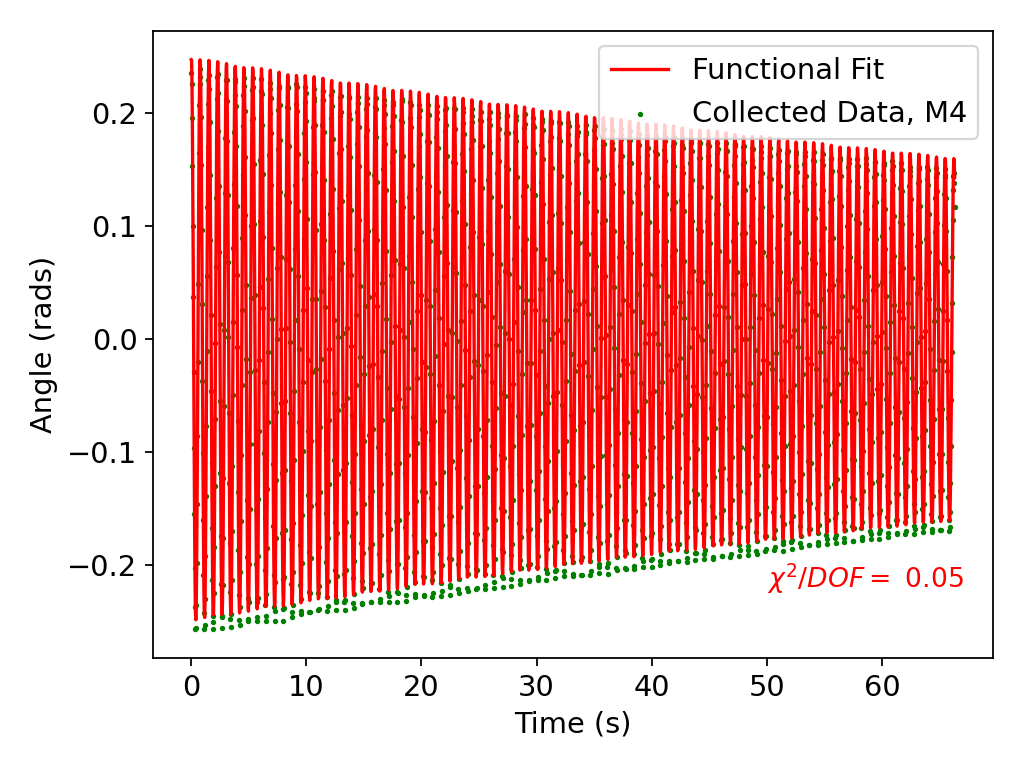
\includegraphics[width=1\textwidth]{Plots/M4.png}
  \caption{\small{$L = 0.10\text{m}$, $m = 0.20\text{kg}$, $\theta_0 = 0.22\text{rads}$}}
  \label{M4}
\end{subfigure}%
\begin{subfigure}[t]{.5\textwidth}
  \centering
  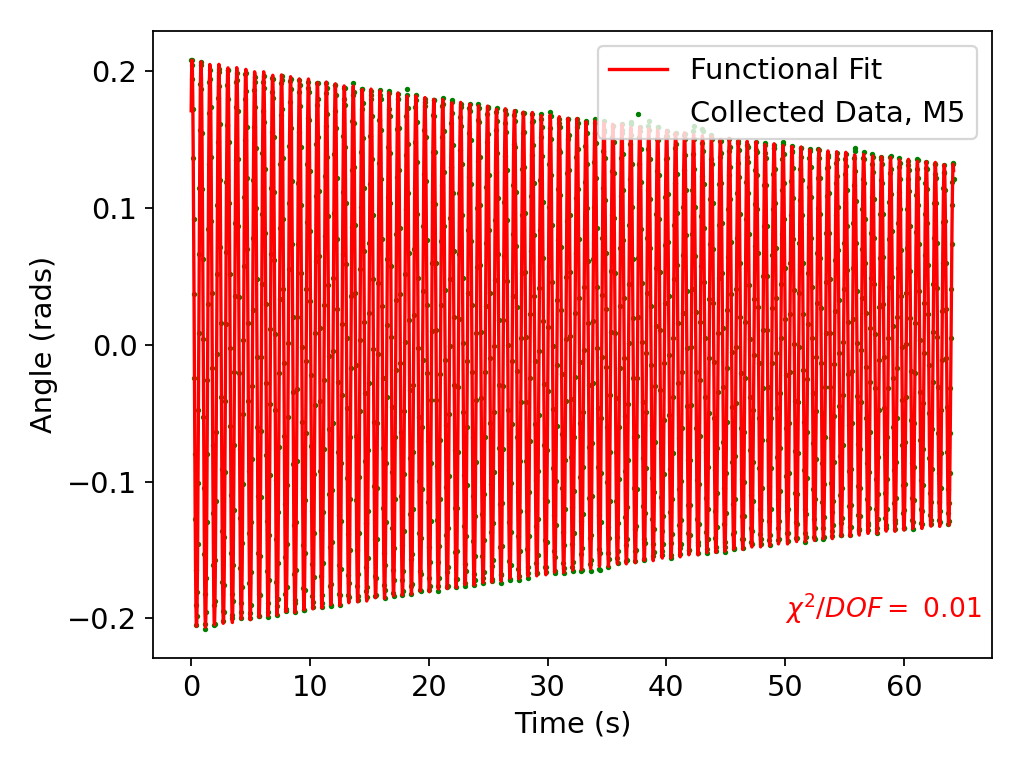
\includegraphics[width=\textwidth]{Plots/M5.png}
  \caption{\small{$L = 0.10\text{m}$, $m = 0.40\text{kg}$, $\theta_0 = 0.22\text{rads}$}}
  \label{M5}
\end{subfigure}
\caption{\small{Plots of the angular amplitude versus time for two systems with independent variables specified above plotted alongside an optimized function of the form Eq.(\ref{theta equation}). Each data set includes over 1 full minute of behaviour of the pendulum.}}
\end{figure}


\begin{figure}[H]
\centering
\begin{subfigure}[t]{0.5\textwidth}
  \centering
  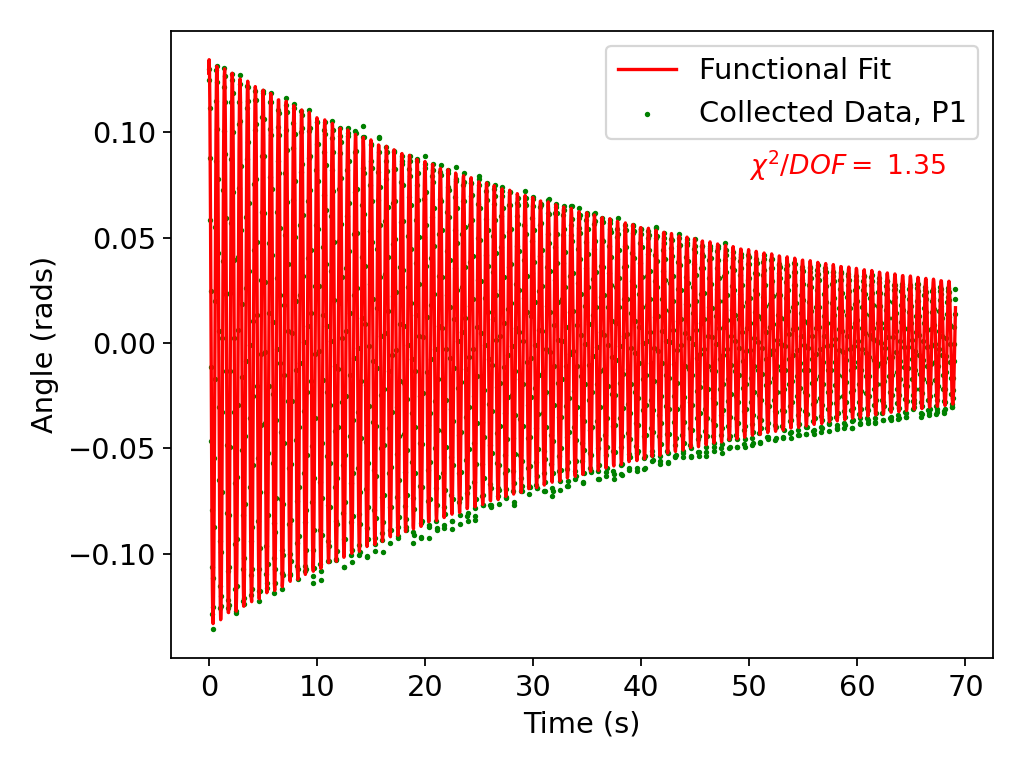
\includegraphics[width=1\textwidth]{Plots/P1.png}
  \caption{\small{$L = 0.10\text{m}$, $m = 0.05\text{kg}$, $\theta_0 = 0.13\text{rads}$}}
  \label{P1}
\end{subfigure}%
\begin{subfigure}[t]{.5\textwidth}
  \centering
  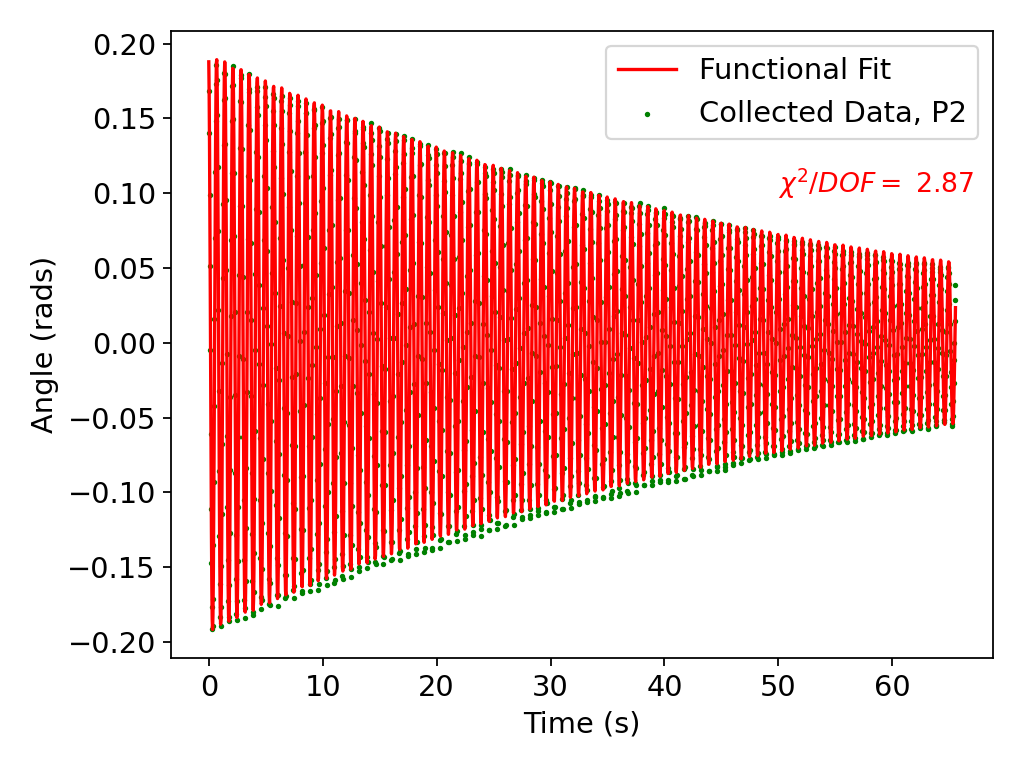
\includegraphics[width=\textwidth]{Plots/P2.png}
  \caption{\small{$L = 0.10\text{m}$, $m = 0.05\text{kg}$, $\theta_0 = 0.17\text{rads}$}}
  \label{P2}
\end{subfigure}
\caption{\small{Plots of the angular amplitude versus time for two systems with independent variables specified above plotted alongside an optimized function of the form Eq.(\ref{theta equation}). Each data set includes over 1 full minute of behaviour of the pendulum.}}
\end{figure}

\begin{figure}[H]
\centering
\begin{subfigure}[t]{0.5\textwidth}
  \centering
  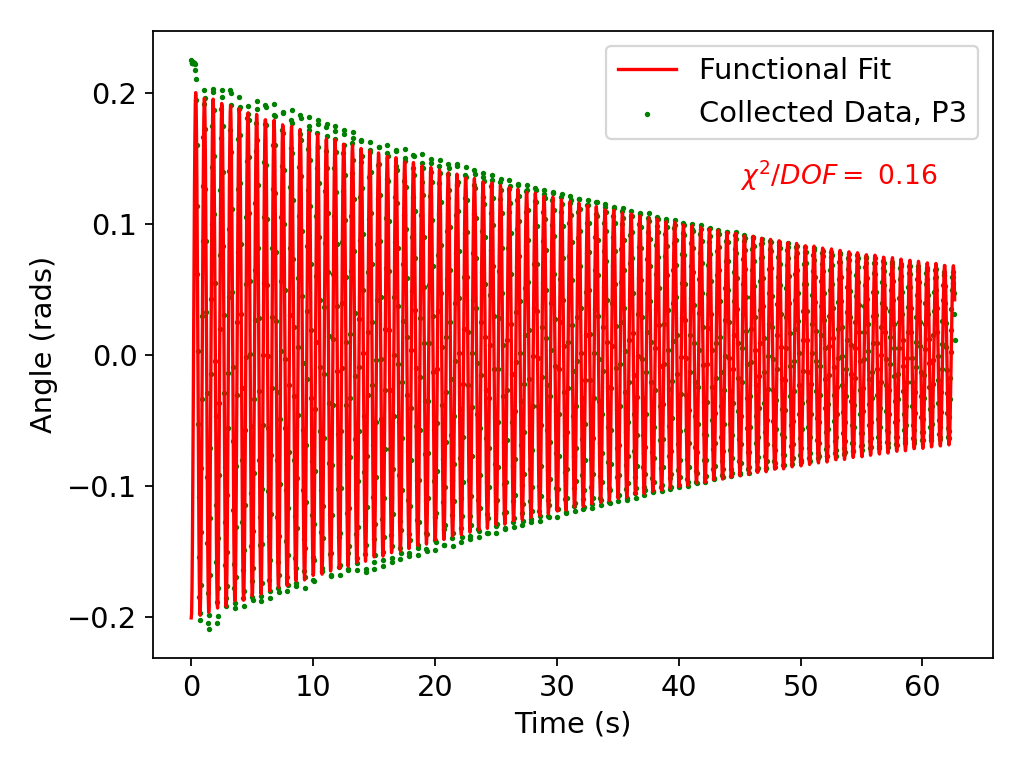
\includegraphics[width=1\textwidth]{Plots/P3.png}
  \caption{\small{$L = 0.10\text{m}$, $m = 0.05\text{kg}$, $\theta_0 = 0.22\text{rads}$}}
  \label{P3}
\end{subfigure}%
\begin{subfigure}[t]{.5\textwidth}
  \centering
  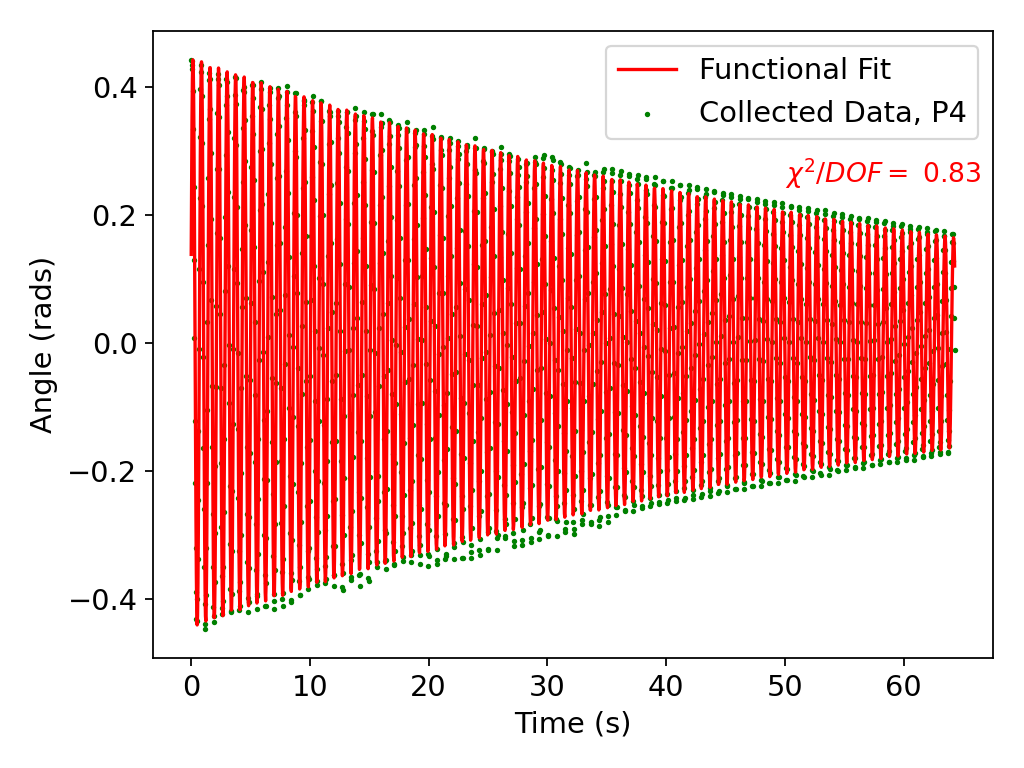
\includegraphics[width=\textwidth]{Plots/P4.png}
  \caption{\small{$L = 0.10\text{m}$, $m = 0.05\text{kg}$, $\theta_0 = 0.44\text{rads}$}}
  \label{P4}
\end{subfigure}
\caption{\small{Plots of the angular amplitude versus time for two systems with independent variables specified above plotted alongside an optimized function of the form Eq.(\ref{theta equation}). Each data set includes over 1 full minute of behaviour of the pendulum.}}
\end{figure}


\begin{figure}[H]
\centering
\begin{subfigure}[t]{0.5\textwidth}
  \centering
  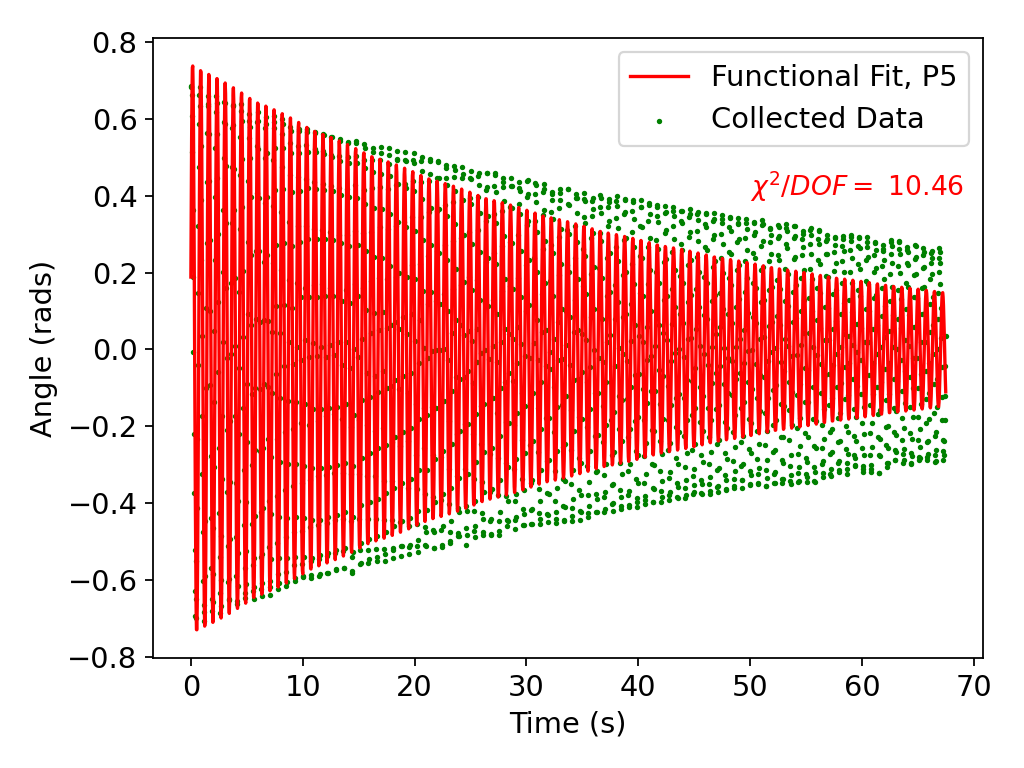
\includegraphics[width=1\textwidth]{Plots/P5.png}
  \caption{\small{$L = 0.10\text{m}$, $m = 0.05\text{kg}$, $\theta_0 = 0.68\text{rads}$}}
  \label{P5}
\end{subfigure}%
\begin{subfigure}[t]{.5\textwidth}
  \centering
  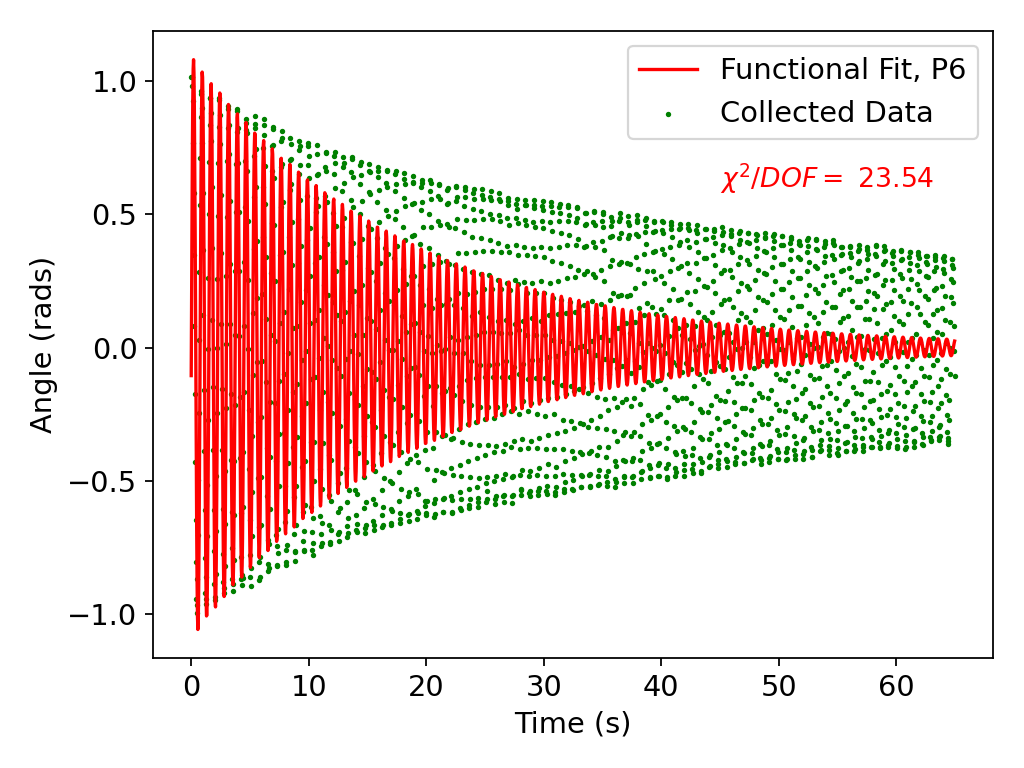
\includegraphics[width=\textwidth]{Plots/P6.png}
  \caption{\small{$L = 0.10\text{m}$, $m = 0.05\text{kg}$, $\theta_0 = 1.02\text{rads}$}}
  \label{P6}
\end{subfigure}
\caption{\small{Plots of the angular amplitude versus time for two systems with independent variables specified above plotted alongside an optimized function of the form Eq.(\ref{theta equation}). Each data set includes over 1 full minute of behaviour of the pendulum.}}
\end{figure}